\section{Highlights of the Coq mechanisation}
\label{sec:coq}

\setminted{fontsize=\footnotesize,linenos=true}

\renewenvironment{mdframed}{}{}

\subsection{Preliminaries}
We begin this section recalling the definition of~$\opMust$, which is given in
\rdef{must-extensional}. It is noteworthy that the mechanised definition, i.e.
\lstinline!must_extensional!, depends on the typeclass \lstinline!Sts!
(\rfig{typeclass-sts}), and {\em not} the type class \lstinline!Lts!. This lays
bare what stated in \rsec{intro}: to define~$\opMust$  a reduction
semantics (i.e. a state transition system), and a predicate $\goodSym$ over
clients suffice.
%% The predicate $\goodSym$ if formalised by the               %%
%% predicate \lstinline!MustT.good! in the Coq code (\rfig{}). %%

\subsubsection{State Transition Systems}

The typeclass for state transition systems (Sts) is defined as follows, where
\mintinline{coq}{A} is the set of states of the Sts. It included a notion of stability
which is axiomatized and decidable.

\begin{mdframed}
\begin{minted}{coq}
Class Sts (A: Type) := {
    sts_step: A → A → Prop;
    sts_state_eqdec: EqDecision A;
    sts_step_decidable: RelDecision sts_step;

    sts_stable: A → Prop;
    sts_stable_decidable p : Decision (sts_stable p);
    sts_stable_spec1 p : ¬ sts_stable p -> { q | sts_step p q };
    sts_stable_spec2 p : { q | sts_step p q } → ¬ sts_stable p;
  }.
\end{minted}
\label{fig:typeclass-sts}
\end{mdframed}

\subsubsection{Maximal computations}

A computation is maximal if it is infinite or if its last state is stable.
%
Given a state \mintinline{coq}{s}, the type \lstinline|max_exec_from s| contains all
the maximal traces that start from \mintinline{coq}{s}. Note the use of a coinductive
type to allow for infinite executions.

\begin{mdframed}
\begin{minted}{coq}
Context `{Sts A}.

CoInductive max_exec_from: A -> Type :=
 | MExStop s (Hstable: sts_stable s) : max_exec_from s
 | MExStep s s' (Hstep: sts_step s s') (η: max_exec_from s') :
    max_exec_from s.
\end{minted}
\end{mdframed}

\leaveout{
\pl{%
\lstinline!max_exec_from! assumes an STS defined on states of type A. It is done with \lstinline!Context `{Sts A}!.
In the definition of \lstinline!must_extensional!, we use \lstinline!max_exec_from! with pairs $(\server,\client)$.
Coq will try to find a way to compose two \lstinline!LTS A L! and \lstinline!LTS B L! to get a \lstinline!LTS (A * B) L!.
It is done using the instance \lstinline!parallel_lts! together with the cast \lstinline!sts_of_lts! from TransitionSystems.v.
Finally, \lstinline!parallel_lts! relies on \lstinline!parallel_steps!.
}
}

\subsection{The must-preorder}
\subsubsection{Client satisfaction}

The predicate $\goodSym$ is defined as any predicate over the states
of an LTS that satisfies certain properties: it is preserved by
structural congruence, by outputs in both directions
(if $p \st{\co{a}} p'$ then $\good{p} \Leftrightarrow \good{p'}$).

It is defined as a typeclass indexed over the type of states and
labels, because we expect a practitioner %that a given LTS has a
to reason on a single canonical notion of "good" at a time.

\begin{mdframed}
\begin{minted}{coq}

Class Good (A L : Type) `{Lts A L, ! LtsEq A L} := {
    good : A -> Prop;
    good_preserved_by_eq p q : good p -> p ≡ q -> good q;
    good_preserved_by_lts_output p q a :
      p ⟶[ActOut a] q -> good p -> good q;
    good_preserved_by_lts_output_converse p q a :
      p ⟶[ActOut a] q -> good q -> good p
}.

\end{minted}
\end{mdframed}

\subsubsection{Must testing}

\rdef{must-extensional}: We write $\Must{\server}{\client} $ if every maximal
  computation of $\csys{\server}{\client}$ is successful.

Given an integer \mintinline{coq}{n} and a maximal execution $\eta$, the function
\lstinline|mex_take_from n| applied to $\eta$ returns \mintinline{coq}{None} if $\eta$
is shorter than \mintinline{coq}{n} and \lstinline|Some p|, where \mintinline{coq}{p} is a
finite execution corresponding to the first \mintinline{coq}{n} steps of $\eta$.

Then, we define the extensional version of $\Must{p}{e}$ by stating that, for
all maximal executions~$\eta$ starting from $(p, e)$, there exists an integer
$n$ such that the $n$-th element of $\eta$ is good.
%
The $n$th element is obtained by taking the last element of the finite prefix of
length~$n$ computed using the function above.

\begin{mdframed}
\begin{minted}{coq}
Context `{good : B -> Prop}.

Fixpoint mex_take_from (n: nat) {x} (η: max_exec_from x) :
  option (finexec_from x) :=
 match n with
  | 0 => Some $ FExSingl x
  | S n => match η with
            | MExStop x Hstable => None
            | MExStep x x' Hstep η' =>
                let p' := mex_take_from n η' in
                (λ p', FExStep x x' (bool_decide_pack _ Hstep) p') <$> p'
           end
 end.

Definition must_extensional (p : A) (e : B) : Prop :=
  forall η : max_exec_from (p, e), exists n fex,
    mex_take_from n η = Some fex /\ good (fex_from_last fex).2.
\end{minted}
\end{mdframed}

\subsubsection{The preorder}

Definition~\ref{def:testleq} is mechanised in a straightforward way:

\begin{mdframed}
%% Finite image write about it
\begin{minted}{coq}
Definition pre_extensional (p : A) (q : R) : Prop :=
   forall (r : B), must_extensional p r -> must_extensional q r.

Notation "p ⊑ₑ q" := (pre_extensional p q).
\end{minted}
\end{mdframed}


\subsection{Behavioural characterizations}

\subsubsection{Labeled Transition Systems}

An LTS is a typeclass indexed by the type of states and the type of labels. The
type of labels must be equipped with decidable equality and be countable, as
enforced by the \mintinline{coq}{Label} typeclass.
%
An action \lstinline|a : Act L| is either an internal action $\tau$ or an external
action: an input or an output of a label in \mintinline{coq}{L}.

\begin{mdframed}
\begin{minted}{coq}
Class Label (L: Type) := {
  label_eqdec: EqDecision L;
  label_countable: Countable L;
}.

Inductive Act (A: Type) := ActExt (μ: ExtAct A) | τ.

Class Lts (A L : Type) `{Label L} := {
    lts_step: A → Act L → A → Prop;
    lts_state_eqdec: EqDecision A;

    lts_step_decidable a α b : Decision (lts_step a α b);

    lts_outputs : A -> gset L;
    lts_outputs_spec1 p1 x p2 :
      lts_step p1 (ActExt (ActOut x)) p2 -> x ∈ lts_outputs p1;
    lts_outputs_spec2 p1 x :
      x ∈ lts_outputs p1 -> {p2 | lts_step p1 (ActExt (ActOut x)) p2};

    lts_stable: A → Act L → Prop;
    lts_stable_decidable p α : Decision (lts_stable p α);
    lts_stable_spec1 p α : ¬ lts_stable p α → { q | lts_step p α q };
    lts_stable_spec2 p α : { q | lts_step p α q } → ¬ lts_stable p α;
  }.

Notation "p ⟶ q"      := (lts_step p τ q).
Notation "p ⟶{ α } q" := (lts_step p α q).
Notation "p ⟶[ α ] q" := (lts_step p (ActExt μ) q).
\end{minted}
\end{mdframed}

An LTS $L$ is cast into an STS by taking only the~$\tau$-transitions, as
formalised by the following instance, which says that \mintinline{coq}{A} can be
equipped with an STS structure when, together with some labels \mintinline{coq}{L},
\mintinline{coq}{A} is equipped with a LTS structure.

\begin{mdframed}
\begin{minted}{coq}
Program Instance sts_of_lts `{Label L} (M: Lts A L): Sts A :=
  {|
    sts_step p q := sts_step p τ q;
    sts_stable s := lts_stable s τ;
  |}.
\end{minted}
\end{mdframed}

\subsubsection{Weak transitions}

Let ${\wt{}} \subseteq \States \times \Actfin \times \States$ denote the least relation such that:
  \begin{description}
  \item[\rname{wt-refl}] $\state \wt{\varepsilon} \stateA$,
  \item[\rname{wt-tau}] $\state \wt{ \trace } \stateB$ if $\state \st{\tau} \stateA$,
    and $\stateA \wt{ \trace } \stateB$
  \item[\rname{wt-mu}]  $\state \wt{\mu.s} \stateB$ if $\state \st{\mu} \stateA$
    and $\stateA \wt{\trace} \stateB$.
  \end{description}


\begin{mdframed}
\begin{minted}{coq}
Definition trace L := list (ExtAct L).

Inductive wt : A -> trace L -> A -> Prop :=
| wt_nil p : wt p [] p
| wt_tau s p q t (l : p ⟶ q) (w : wt q s t) : wt p s t
| wt_act μ s p q t (l : p ⟶[μ] q) (w : wt q s t) : wt p (μ :: s) t.

Notation "p ⟹[s] q" := (wt p s q).
\end{minted}
\end{mdframed}

\subsubsection{Product of LTS}

The characteristic function of the transition relation of the
LTS resulting from the parallel composition of two LTS.
%
States of the parallel product of $L_1$ and $L_2$ are pairs $(a, b) \in L_1
\times L_2$.
%
The first two cases correspond to unsynchronized steps from either LTS, and the
third case corresponds to the LTS taking steps with dual actions. The predicate
\lstinline|act_match l1 l2| states that the two actions are visible and are dual
of each other.

\begin{mdframed}
\begin{minted}{coq}
Inductive parallel_step `{M1: Lts A L, M2: Lts B L} :
  A * B → Act L → A * B → Prop :=
| ParLeft l a1 a2 b: a1 -[l]→ a2 → parallel_step (a1, b) l (a2, b)
| ParRight l a b1 b2: b1 -[l]→ b2 → parallel_step (a, b1) l (a, b2)
| ParSync l1 l2 a1 a2 b1 b2:
  act_match l1 l2 → a1 -[l1]→ a2 → b1 -[l2]→ b2 →
  parallel_step (a1, b1) τ (a2, b2)
.
\end{minted}
\end{mdframed}


\begin{figure}
  \hrulefill
\begin{center}
  \scalebox{.9}{%
    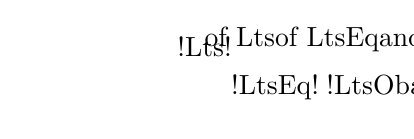
\begin{tikzpicture}
      \node (Lts) {\lstinline!Lts!};
      \node (LtsEq) [below =+7pt of Lts]  {\lstinline!LtsEq!};
      \node (LtsOba) [below =+7pt of LtsEq]  {\lstinline!LtsOba!};
      \node (LtsFb) [below left=+7pt and +1pt of LtsOba]  {\lstinline!LtsObaFb!};
      \node (LtsFw) [below right=+7pt and +1pt of LtsOba]  {\lstinline!LtsObaFw!};

      \path[->]
      (Lts) edge (LtsEq)
      (LtsEq) edge (LtsOba)
      (LtsOba) edge (LtsFb)
      (LtsOba) edge (LtsFw);
    \end{tikzpicture}
  }
\end{center}
%  \vspace{-10pt}
  \caption{Typeclasses to formalise LTSs.}
  \hrulefill
  \label{fig:structure-typeclasses-lts}
\end{figure}


\subsection{Typeclasses for LTS}
The Selinger axioms for LTSs are represented as three typeclasses in our Coq
development.

\begin{mdframed}
  \begin{minted}{coq}
Class LtsOba (A L : Type) `{Lts A L, !LtsEq A L} :=
    MkOBA {
      lts_oba_output_commutativity {p q r a α} :
        p ⟶[ActOut a] q → q ⟶{α} r →
        ∃ t, p ⟶{α} t ∧ t ⟶≡[ActOut a] r ;
      lts_oba_output_confluence {p q1 q2 a μ} :
        μ ≠ ActOut a → p ⟶[ActOut a] q1 → p ⟶[μ] q2 →
        ∃ r, q1 ⟶[μ] r ∧ q2 ⟶≡[ActOut a] r ;
      lts_oba_output_tau {p q1 q2 a} :
        p ⟶[ActOut a] q1 → p ⟶ q2 →
        (∃ t, q1 ⟶ t ∧ q2 ⟶≡[ActOut a] t) ∨ q1 ⟶≡[ActIn a] q2 ;
      lts_oba_output_deter {p1 p2 p3 a} :
        p1 ⟶[ActOut a] p2 → p1 ⟶[ActOut a] p3 → p2 ≡ p3 ;
      lts_oba_output_deter_inv {p1 p2 q1 q2} a :
        p1 ⟶[ActOut a] q1 → p2 ⟶[ActOut a] q2 → q1 ≡ q2 → p1 ≡ p2;
      (* Multiset of outputs *)
      lts_oba_mo p : gmultiset L;
      lts_oba_mo_spec1 p a : a ∈ lts_oba_mo p <-> a ∈ lts_outputs p;
      lts_oba_mo_spec2 p a q :
        p ⟶[ActOut a] q -> lts_oba_mo p = {[+ a +]} ⊎ lts_oba_mo q;
    }.

Class LtsObaFB (A L: Type) `{LtsOba A L} :=
  MkLtsObaFB {
      lts_oba_fb_feedback {p1 p2 p3 a} :
        p1 ⟶[ActOut a] p2 → p2 ⟶[ActIn a] p3 → p1 ⟶≡ p3
    }.

Class LtsObaFW (A L : Type) `{LtsOba A L} :=
  MkLtsObaFW {
      lts_oba_fw_forward p1 a :
        ∃ p2, p1 ⟶[ActIn a] p2 ∧ p2 ⟶≡[ActOut a] p1;
      lts_oba_fw_feedback {p1 p2 p3 a} :
        p1 ⟶[ActOut a] p2 → p2 ⟶[ActIn a] p3 → p1 ⟶≡ p3 ∨ p1 ≡ p3;
    }.
  \end{minted}
\end{mdframed}

\subsubsection{Termination}

We write $\state \conv$ and say that {\em $\state$ converges} if every
sequence of $\tau$-transitions performed by $\state$ is finite. This is
expressed extensionally by the property that all maximal computations starting
from $p$ contain a \emph{stable} process, meaning that it is finite.

\begin{mdframed}
\begin{minted}{coq}
Definition terminate (p : A) : Prop :=
    forall η : max_exec_from p, exists n fex,
      mex_take_from n η = Some fex /\ lts_stable (fex_from_last fex) τ.
\end{minted}
\end{mdframed}

\subsubsection{Convergence along a trace}

To define the behavioural characterisation of the preorder, we first define
${\cnvalong} \subseteq \States \times \Actfin$ as the least relation such
that,% (\coqConv{cnv}),h
\begin{description}
\item[\cnvepsilon] $\state \cnvalong \varepsilon$ if $\state \conv$,
\item[\cnvmu] $ \state \cnvalong \mu.\trace $ if $p \conv$ and for each $\stateA$,
$\state \wt{\mu} \stateA \implies \stateA \cnvalong \trace$.
\end{description}

\noindent
This corresponds to the following inductive predicate in Coq:

\begin{mdframed}
\begin{minted}{coq}
Inductive cnv : A -> trace L -> Prop :=
  | cnv_ext_nil p : terminate p -> cnv p []
  | cnv_ext_act p μ s :
    terminate p -> (forall q, p ⟹{μ} q -> cnv q s) -> cnv p (μ :: s).

Notation "p ⇓ s" := (cnv p s).
\end{minted}
\end{mdframed}


\subsection{Forwarders}

We define a mailbox $MO$ as a multiset of names.

\begin{mdframed}
\begin{minted}{coq}
Definition mb (L : Type) `{Label L} := gmultiset L.
\end{minted}
\end{mdframed}

\noindent
\rdef{liftFW} and \rfig{rules-liftFW}\emph{
Lifting of a transition relation to transitions of forwarders.
}

\begin{mdframed}
\begin{minted}{coq}
Inductive lts_fw_step {A L : Type} `{Lts A L} :
  A * mb L -> Act L -> A * mb L -> Prop :=
| lts_fw_p p q m α:
  lts_step p α q -> lts_fw_step (p ▷ m) α (q ▷ m)
| lts_fw_out_mb m p a :
  lts_fw_step (p ▷ {[+ a +]} ⊎ m) (ActExt $ ActOut a) (p ▷ m)
| lts_fw_inp_mb m p a :
  lts_fw_step (p ▷ m) (ActExt $ ActIn a) (p ▷ {[+ a +]} ⊎ m)
| lts_fw_com m p a q :
  lts_step p (ActExt $ ActIn a) q ->
  lts_fw_step (p ▷ {[+ a +]} ⊎ m) τ (q ▷ m).
\end{minted}
\end{mdframed}

\noindent
\rdef{strip-def} and \rdef{fw-eq}\emph{
For any LTS $\genlts$,
two states of $\liftFW{\genlts}$ are equivalent, denoted
$\serverA \triangleright M \doteq \serverB \triangleright N$, if
$ \strip{ \serverA } \simeq \strip{ \serverB }$
and $M \uplus \outputmultiset{\serverA} = N \uplus \outputmultiset{\serverB}$.
}

\begin{mdframed}
\begin{minted}{coq}
Inductive strip `{Lts A L} : A -> gmultiset L -> A -> Prop :=
| strip_nil p : p ⟿{∅} p
| strip_step p1 p2 p3 a m :
  p1 ⟶[ActOut a] p2 -> p2 ⟿{m} p3 -> p1 ⟿{{[+ a +]} ⊎ m} p3

where "p ⟿{ m } q" := (strip p m q).

Definition fw_eq `{LtsOba A L} (p : A * mb L) (q : A * mb L) :=
  forall (p' q' : A),
    p.1 ⟿{lts_oba_mo p.1} p' ->
    q.1 ⟿{lts_oba_mo q.1} q' ->
    p' ⋍ q' /\ lts_oba_mo p.1 ⊎ p.2 = lts_oba_mo q.1 ⊎ q.2.

Infix "≐" := fw_eq (at level 70).
\end{minted}
\end{mdframed}

\noindent
\rlem{harmony-sta}\emph{
For every $\genlts_\StatesA$ and every
$\serverA \triangleright M, \serverB \triangleright N \in \StatesA \times MO$,
and every $\alpha \in L$, if
$
\serverA \triangleright M \mathrel{({\doteq} \cdot {\sta{\alpha}})}
\serverB \triangleright N
$ then
$
\serverA  \triangleright M \mathrel{({\sta{\alpha}} \cdot {\doteq})} \serverB' \triangleright N'.
$
}

\begin{mdframed}
\begin{minted}{coq}
Lemma lts_fw_eq_spec `{LtsObaFB A L} p q t mp mq mt α :
  p ▷ mp ≐ t ▷ mt -> (t ▷ mt) ⟶{α} (q ▷ mq) -> p ▷ mp ⟶≐{α} q ▷ mq.
\end{minted}
\end{mdframed}

\noindent
\rlem{liftFW-works}. \emph{For every LTS~$\genlts \in \obaFB$, $\liftFW{\genlts}
\in \obaFW$.}

\begin{mdframed}
\begin{minted}{coq}
Program Instance LtsMBObaFW `{LtsObaFB A L} : LtsObaFW (A * mb L) L.
\end{minted}
\end{mdframed}


\noindent
\rlem{musti-obafb-iff-musti-obafw}\emph{
For every $\genlts_A, \genlts_B \in \obaFB, \server \in A, \client \in B$,
$\musti{\server}{\client}$ if and only if $\musti{\liftFW{\server}}{\client}$.
}

\begin{mdframed}
\begin{minted}{coq}
Lemma must_iff_must_fw
  {@LtsObaFB A L IL LA LOA V, @LtsObaFB B L IL LB LOB W,
   !FiniteLts A L, !Good B L good }
  (p : A) (e : B) : must p e ↔ must (p, ∅) e.
\end{minted}
\end{mdframed}

\subsection{The Acceptance Set Characterisation}

The behavioural characterisation with acceptance sets
(Definition~\ref{def:accset-leq}) is formalised as follows.
%
Note that \mintinline{coq}{lts_outputs}, used in the second part of the definition, is
part of the definition of an \mintinline{coq}{Lts}, and produces the finite set of
outputs that a process can immediately produce.

\begin{mdframed}
\begin{minted}{coq}
Definition bhv_pre_cond1 `{Lts A L, Lts B L} (p : A) (q : B) :=
  forall s, p ⇓ s -> q ⇓ s.

Notation "p ≼₁ q" := (bhv_pre_cond1 p q) (at level 70).

Definition bhv_pre_cond2 `{Lts A L, Lts B L} (p : A) (q : B) :=
  forall s q', p ⇓ s -> q ⟹[s] q' -> q' ↛ ->
    ∃ p', p ⟹[s] p' /\ p' ↛ /\ lts_outputs p' ⊆ lts_outputs q'.

Notation "p ≼₂ q" := (bhv_pre_cond2 p q) (at level 70).

Definition bhv_pre `{@Lts A L HL, @Lts B L HL} (p : A) (q : B) :=
  p ≼₁ q /\ p ≼₂ q.

Notation "p ≼ q" := (bhv_pre p q) (at level 70).
\end{minted}
\end{mdframed}

Given an LTS that satisfies the right conditions, \mustequivalence coincides
with the behavioural characterisation above on the LTS of forwarders
(Theorem~\ref{thm:testleqS-equals-bhvleq}).

\begin{mdframed}
\begin{minted}{coq}
Section correctness.
  Context `{LtsObaFB A L, LtsObaFB R L, LtsObaFB B L}.
  Context `{!FiniteLts A L, !FiniteLts B L, !FiniteLts R L, !Good B L}.
  (* The LTS can express the tests required for completeness *)
  Context `{!gen_spec_conv gen_conv, !gen_spec_acc gen_acc}.

  Theorem equivalence_bhv_acc_ctx (p : A) (q : R) :
    p ⊑ₑ q <-> (p, ∅) ≼ (q, ∅).
End correctness.
\end{minted}
\end{mdframed}

\subsection{The Must Set characterisation}

The behavioural characterisation with must sets
(Definition~\ref{def:denicola-char}) is formalised as follows.

\begin{mdframed}
  \begin{minted}{coq}
Definition MUST `{Lts A L} (p : A) (G : gset (ExtAct L)) :=
    forall p', p ⟹ p' -> exists μ p0, μ ∈ G /\ p' ⟹{μ} p0.

Definition MUST__s `{FiniteLts A L} (ps : gset A) (G : gset (ExtAct L)) :=
  forall p, p ∈ ps -> MUST p G.

Definition AFTER `{FiniteLts A L} (p : A) (s : trace L) (hcnv : p ⇓ s) :=
  wt_set p s hcnv.

Definition bhv_pre_ms_cond2
  `{@FiniteLts A L HL LtsA, @FiniteLts B L HL LtsB} (p : A) (q : B) :=
  forall s h1 h2 G, MUST__s (AFTER p s h1) G -> MUST__s (AFTER q s h2) G.

Notation "p ≾₂ q" := (bhv_pre_ms_cond2 p q) (at level 70).

Definition bhv_pre_ms `{@FiniteLts A L HL LtsA, @FiniteLts B L HL LtsB}
  (p : A) (q : B) := p ≼₁ q /\ p ≾₂ q.

Notation "p ≾ q" := (bhv_pre_ms p q).
  \end{minted}
\end{mdframed}


\noindent
\rlem{acceptance-sets-and-must-sets-have-same-expressivity}\emph{
Let $\genlts_A, \genlts_B \in \obaFB$.
For every $\serverA \in \StatesA$  and
$\serverB \in \StatesB $ such that $\liftFW{ \serverA } \bhvleqone \liftFW{ \serverB }$,
we have that
$\liftFW{ \serverA } \msleqtwo \liftFW{ \serverB }$ if and only if
$\liftFW{ \serverA } \asleqAfw \liftFW{ \serverB }$.
}

\begin{mdframed}
\begin{minted}{coq}
Context `{@LtsObaFB A L LL LtsA LtsEqA LtsObaA}.
Context `{@LtsObaFB B L LL LtsR LtsEqR LtsObaR}.

Lemma equivalence_bhv_acc_mst2 (p : A) (q : B) :
  (p, ∅) ≼₁ (q, ∅) -> (p, ∅) ≾₂ (q, ∅) <-> (p, ∅) ≼₂ (q, ∅).
\end{minted}
\end{mdframed}

Given an LTS that satisfies the right conditions, \mustequivalence coincides
with the behavioural characterisation above on the LTS of forwarders
(Theorem~\ref{thm:testleqS-equals-mustsetleq}).

\begin{mdframed}
\begin{minted}{coq}
Section correctness.
  Context `{LtsObaFB A L, LtsObaFB R L, LtsObaFB B L}.
  Context `{!FiniteLts A L, !FiniteLts B L, !FiniteLts R L, !Good B L}.
  (* The LTS can express the tests required for completeness. *)
  Context `{!gen_spec_conv gen_conv, !gen_spec_acc gen_acc}.

  Theorem equivalence_bhv_mst_ctx (p : A) (q : R) :
    p ⊑ₑ q <-> (p, ∅) ≾ (q, ∅).
End correctness.
\end{minted}
\end{mdframed}

\subsection{From extensional to intensional definitions}

\rprop{ext-impl-int}\emph{
Given a countably branching STS~$\sts{\SysStates}{\to}$, and a decidable predicate~$Q$
on~$\SysStates$, for all~$s \in \SysStates$, $\mathsf{ext}_Q(s)$ implies
$\mathsf{int}_Q(s).$
}

\begin{mdframed}
\begin{minted}{coq}
Context `{Hsts: Sts A, @CountableSts A Hsts}.
Context `{@Bar A Hsts}.

Theorem extensional_implies_intensional x:
  extensional_pred x -> intensional_pred x.
\end{minted}
\end{mdframed}

\rcor{ext-int-eq-conv}\emph{
For every $\server \in \States$,
\begin{enumerate}
\item $\state \conv $ if and only if $\state \convi$,
\item for every $\client$ we have that $\Must{\server}{\client}$ if
  and only if $\musti{\server}{\client}$.
\end{enumerate}
}

\begin{mdframed}
\begin{minted}{coq}
Context `{Label L}.
Context `{!Lts A L, !FiniteLts A L}.

Lemma terminate_extensional_iff_terminate (p : A) :
  terminate_extensional p <-> terminate p.

Inductive must_sts `{Sts (A * B), good : B -> Prop} (p : A) (e : B) :
  Prop :=
| m_sts_now : good e -> must_sts p e
| m_sts_step
    (nh : ¬ good e)
    (nst : ¬ sts_stable (p, e))
    (l : forall p' e', sts_step (p, e) (p', e') -> must_sts p' e')
  : must_sts p e
.

Lemma must_extensional_iff_must_sts
  `{good : B -> Prop, good_decidable : forall (e : B), Decision (good e)}
  `{Lts A L, !Lts B L, !LtsEq B L, !Good B L good,
    !FiniteLts A L, !FiniteLts B L} (p : A) (e : B) :
  must_extensional p e <-> must_sts p e.
\end{minted}
\end{mdframed}

Equivalence between the inductive definitions of $\opMust$ defined using Sts and $\opMust$ defined using Lts.

\begin{mdframed}
\begin{minted}{coq}
Inductive must `{Lts A L, !Lts B L, !LtsEq B L, !Good B L good}
  (p : A) (e : B) : Prop :=
| m_now : good e -> must p e
| m_step
    (nh : ¬ good e)
    (ex : ∃ t, parallel_step (p, e) τ t)
    (pt : forall p', p ⟶ p' -> must p' e)
    (et : forall e', e ⟶ e' -> must p e')
    (com : forall p' e' μ, e ⟶[μ] e' -> p ⟶[co μ] p' -> must p' e')
  : must p e
.

Lemma must_sts_iff_must `{Lts A L, !Lts B L, !LtsEq B L, !Good B L good}
  (p : A) (e : B) : must_sts p e <-> must p e.
\end{minted}
\end{mdframed}



\subsection{Completeness}

Properties of the functions that generate clients (\rtab{properties-functions-to-generate-clients}).

\begin{mdframed}
\begin{minted}{coq}
Class gen_spec {A L : Type} `{Lts A L, !LtsEq A L, !Good A L good}
  (gen : list (ExtAct L) -> A) := {
    gen_spec_ungood : forall s, ¬ good (gen s) ;
    gen_spec_mu_lts_co μ s : gen (μ :: s) ⟶⋍[co μ] gen s;
    gen_spec_out_lts_tau_ex a s : ∃ e', gen (ActOut a :: s) ⟶ e';
    gen_spec_out_lts_tau_good a s e : gen (ActOut a :: s) ⟶ e -> good e;
    gen_spec_out_lts_mu_uniq {e a μ s} :
    gen (ActOut a :: s) ⟶[μ] e -> e = gen s /\ μ = ActIn a;
  }.

Class gen_spec_conv {A L : Type} `{Lts A L, ! LtsEq A L, !Good A L good}
  (gen_conv : list (ExtAct L) -> A) := {
    gen_conv_spec_gen_spec : gen_spec gen_conv ;
    gen_spec_conv_nil_stable_mu μ : gen_conv [] ↛[μ] ;
    gen_spec_conv_nil_lts_tau_ex : ∃ e', gen_conv [] ⟶ e';
    gen_spec_conv_nil_lts_tau_good e : gen_conv [] ⟶ e -> good e;
  }.

Class gen_spec_acc {A : Type} `{Lts A L, ! LtsEq A L, !Good A L good}
  (gen_acc : gset L -> list (ExtAct L) -> A) := {
    gen_acc_spec_gen_spec O : gen_spec (gen_acc O);
    gen_spec_acc_nil_stable_tau O : gen_acc O [] ↛;
    gen_spec_acc_nil_stable_out O a : gen_acc O [] ↛[ActOut a];
    gen_spec_acc_nil_mu_inv O a e : gen_acc O [] ⟶[ActIn a] e -> a ∈ O;
    gen_spec_acc_nil_mem_lts_inp O a :
      a ∈ O -> ∃ r, gen_acc O [] ⟶[ActIn a] r;
    gen_spec_acc_nil_lts_inp_good μ e' O :
      gen_acc O [] ⟶[μ] e' -> good e';
  }.
\end{minted}
\end{mdframed}

\noindent
\rprop{must-iff-acnv}\emph{
For every $\genlts_{\States} \in \obaFW$,
$\server \in \States$, and
$\trace \in \Actfin$ we have that $\musti{\server}{ \testconv{ \trace} }$
if and only if~$\server \cnvalong \trace$.
}

\begin{mdframed}
\begin{minted}{coq}
Lemma must_iff_cnv
  `{@LtsObaFW A L IL LA LOA V, @LtsObaFB B L IL LB LOB W,
    !Good B L good, !gen_spec_conv gen_conv} (p : A) s :
   must p (gen_conv s) <-> p ⇓ s.
Proof. split; [eapply cnv_if_must | eapply must_if_cnv]; eauto. Qed.
\end{minted}
\end{mdframed}

\noindent
\rlem{must-output-swap-l-fw}\emph{
  Let $\genlts_A \in \obaFW$ and
  $\genlts_B \in \obaFB$.
  $\Forevery \serverA_1, \serverA_2 \in \StatesA$,
  every $\client_1, \client_2 \in \StatesB$ and name $\aa \in \Names$ such that
  $\serverA_1 \st{\co{\aa}} \serverA_2$ and
  $\client_1 \st{\co{\aa}} \client_2$,
  if $\musti{\serverA_1}{\client_2}$ then $\musti{\serverA_2}{\client_1}$.
}

\begin{mdframed}
\begin{minted}{coq}
Lemma must_output_swap_l_fw
  `{@LtsObaFW A L IL LA LOA V, @LtsObaFB B L IL LB LOB W, !Good B L good}
  (p1 p2 : A) (e1 e2 : B) (a : L) :
  p1 ⟶[ActOut a] p2 -> e1 ⟶[ActOut a] e2 -> must p1 e2 -> must p2 e1.
\end{minted}
\end{mdframed}

\noindent
\rlem{completeness-part-2.2-diff-outputs}.\emph{
Let $\genlts_A \in \obaFW$.
For every $\server \in \States$, $\trace \in \Actfin$,
and every $L, E \subseteq \Names$, if
$\co{L} \in \accht{ \server }{ \trace }$
then $\Nmusti{ \server }{ \testacc{\trace}{E \setminus L}}$.
}

\begin{mdframed}
\begin{minted}{coq}
Lemma not_must_gen_a_without_required_output
  `{@LtsObaFW A L IL LA LOA V, @LtsObaFB B L IL LB LOB W,
    !Good B L good, !gen_spec_acc gen_acc} (q q' : A) s O :
  q ⟹[s] q' -> q' ↛ -> ¬ must q (gen_acc (O ∖ lts_outputs q') s).
\end{minted}
\end{mdframed}

\noindent
\rlem{completeness-part-2.2-auxiliary}\emph{
Let $\genlts_A \in \obaFW$.
$\Forevery \server \in \States, \trace \in \Actfin$,
and every finite set $\ohmy \subseteq \co{\Names}$,
if $\server \cnvalong s$ then either
\begin{enumerate}[(i)]
\item
  $\musti{\server}{\testacc{ \trace }{ \bigcup \co{ \accht{p}{s}
      \setminus \ohmy }}}$, or
\item
  there exists $\widehat{\ohmy} \in \accht{ \server }{ \trace }$ such that $\widehat{\ohmy} \subseteq \ohmy$.
\end{enumerate}
}

\begin{mdframed}
\begin{minted}{coq}
Lemma must_gen_a_with_s
  `{@LtsObaFW A L IL LA LOA V, @LtsObaFB B L IL LB LOB W,
    !FiniteLts A L, !Good B L good, !gen_spec_acc gen_acc}
  s (p : A) (hcnv : p ⇓ s) O :
  (exists p', p ⟹[s] p' /\ lts_stable p' τ /\ lts_outputs p' ⊆ O)
    \/ must p (gen_acc (oas p s hcnv ∖ O) s).
\end{minted}
\end{mdframed}

\noindent
\rlem{completeness}.\emph{
For every $\genlts_A, \genlts_B \in \obaFW$ and
servers $\serverA \in \StatesA, \serverB \in \StatesB $,
if ${ \serverA } \testleqS { \serverB }$
then ${ \serverA } \asleq { \serverB }$.
}

\begin{mdframed}
\begin{minted}{coq}
Lemma completeness_fw
  `{@LtsObaFW A L IL LA LOA V, @LtsObaFB B L IL LB LOB W,
    @LtsObaFW C L IL LC LOC VC, !FiniteLts A L, !FiniteLts C L,
    !FiniteLts B L, !Good B L good,
    !gen_spec_conv gen_conv, !gen_spec_acc gen_acc}
  (p : A) (q : C) : p ⊑ q -> p ≼ q.
\end{minted}
\end{mdframed}

\noindent
\rprop{bhv-completeness}.
For every $\genlts_A, \genlts_B \in \obaFB$ and
servers $\serverA \in \StatesA, \serverB \in \StatesB $,
if $\serverA \testleqS \serverB$ then $\liftFW{ \serverA } \asleq \liftFW{ \serverB }$.

\begin{mdframed}
\begin{minted}{coq}
Lemma completeness
  `{@LtsObaFB A L IL LA LOA V, @LtsObaFB B L IL LB LOB W,
    @LtsObaFB C L IL LC LOC VC,
    !FiniteLts A L, !FiniteLts B L, !FiniteLts C L, !Good C L good,
    !gen_spec_conv gen_conv, !gen_spec_acc gen_acc}
  (p : A) (q : B) : p ⊑ q -> p ▷ ∅ ≼ q ▷ ∅.
\end{minted}
\end{mdframed}

\subsection{Soundness}

\rfig{rules-mustset-main}. Rules to define inductively the predicate $\opMustset$.

\begin{mdframed}
\begin{minted}{coq}
Inductive mustx
  `{Lts A L, !FiniteLts A L, !Lts B L, !LtsEq B L, !Good B L good}
  (ps : gset A) (e : B) : Prop :=
| mx_now (hh : good e) : mustx ps e
| mx_step
    (nh : ¬ good e)
    (ex : forall (p : A), p ∈ ps -> ∃ t, parallel_step (p, e) τ t)
    (pt : forall ps',
        lts_tau_set_from_pset_spec1 ps ps' -> ps' ≠ ∅ ->
        mustx ps' e)
    (et : forall (e' : B), e ⟶ e' -> mustx ps e')
    (com : forall (e' : B) μ (ps' : gset A),
        lts_step e (ActExt μ) e' ->
        wt_set_from_pset_spec1 ps [co μ] ps' -> ps' ≠ ∅ ->
        mustx ps' e')
  : mustx ps e.
\end{minted}
\end{mdframed}

\noindent
\rlem{musti-if-mustset-helper}\emph{
For every LTS $\genlts_A, \genlts_B$ and every
$X \in \pparts{\StatesA}$, we have that
$\mustset{X}{\client}$ if and only if for every $\serverA \in X
\wehavethat \musti{\serverA}{\client}$.
}

\begin{mdframed}
\begin{minted}{coq}
Lemma must_set_iff_must_for_all
  `{Lts A L, !FiniteLts A L, !Lts B L, !LtsEq B L, !Good B L good}
  (X : gset A) (e : B) : X ≠ ∅ ->
    (forall p, p ∈ X -> must p e) <-> mustx X e.
\end{minted}
\end{mdframed}

Lifting of the predicates~$\bhvleqone$ and~$\bhvleqtwo$ to sets of servers.

\begin{mdframed}
\begin{minted}{coq}
Definition bhv_pre_cond1__x `{FiniteLts P L, FiniteLts Q L}
 (ps : gset P) (q : Q) := forall s, (forall p, p ∈ ps -> p ⇓ s) -> q ⇓ s.

Notation "ps ≼ₓ1 q" := (bhv_pre_cond1__x ps q) (at level 70).

Definition bhv_pre_cond2__x
  `{@FiniteLts P L HL LtsP, @FiniteLts Q L HL LtsQ}
  (ps : gset P) (q : Q) :=
  forall s q', q ⟹[s] q' -> q' ↛ ->
    (forall p, p ∈ ps -> p ⇓ s) ->
    exists p, p ∈ ps /\ exists p',
      p ⟹[s] p' /\ p' ↛ /\ lts_outputs p' ⊆ lts_outputs q'.

Notation "ps ≼ₓ2 q" := (bhv_pre_cond2__x ps q) (at level 70).

Notation "ps ≼ₓ q" := (bhv_pre_cond1__x ps q /\ bhv_pre_cond2__x ps q)
   (at level 70).
\end{minted}
\end{mdframed}

\noindent
\rlem{alt-set-singleton-iff}.\emph{
For every LTS $\genlts_A, \genlts_B$ and servers $\server \in \StatesA$,
$\serverB \in \StatesB$,
$\serverA \asleq \serverB$ if and only if $\set{\serverA} \asleqset \serverB$.
}


\begin{mdframed}
\begin{minted}{coq}
Lemma alt_set_singleton_iff
  `{@FiniteLts P L HL LtsP, @FiniteLts Q L HL LtsQ}
  (p : P) (q : Q) : p ≼ q <-> {[ p ]} ≼ₓ q.
\end{minted}
\end{mdframed}

\noindent
\rlem{bhvleqone-preserved}.\emph{
Let $\genlts_\StatesA, \genlts_\StatesB \in \obaFW$.
For every set $X \in \pparts{ \StatesA }$, and
$\serverB \in \StatesB$, such that
$X \cnvleqset \serverB$ then
\begin{enumerate}
\item
  $\serverB \st{ \tau } \serverB'$ implies $X \cnvleqset \serverB'$,
\item
  $X \convi$, $X \wt{\mu} X'$ and $\serverB \st{\mu} \serverB'$ imply $X' \cnvleqset \serverB'$.
\end{enumerate}
}

\noindent
\rlem{bhvleqtwo-preserved}\emph{
Let $\genlts_\StatesA, \genlts_\StatesB \in \obaFW$.
For every
$X, X' \in \pparts{ \StatesA }$ and $ \serverB \in \StatesB$,
such that $X \accleqset \serverB$, then
\begin{enumerate}
\item
  $\serverB \st{ \tau } \serverB'$ implies $X \accleqset \serverB'$,
\item
  for every $\mu \in \Act$,
  if $X \convi$, then for every  $\serverB \st{\mu} \serverB'$ and set $X \wt{\mu} X'$
  we have $X' \accleqset \serverB'$.
\end{enumerate}
}

\begin{mdframed}
\begin{minted}{coq}
Lemma bhvx_preserved_by_tau
  `{@FiniteLts P L HL LtsP, @FiniteLts Q L HL LtsQ}
  (ps : gset P) (q q' : Q) : q ⟶ q' -> ps ≼ₓ q -> ps ≼ₓ q'.

Lemma bhvx_preserved_by_mu
  `{@FiniteLts P L HL LtsP, @FiniteLts Q L HL LtsQ}
  (ps0 : gset P) (q : Q) μ ps1 q'
  (htp : forall p, p ∈ ps0 -> terminate p) :
  q ⟶[μ] q' -> wt_set_from_pset_spec ps0 [μ] ps1 ->
  ps0 ≼ₓ q -> ps1 ≼ₓ q'.
\end{minted}
\end{mdframed}

\noindent
Lemma \emph{
Let $\genlts_\StatesA, \genlts_\StatesB \in \obaFW$ and $\genlts_\StatesC \in \obaFB$.
For every $X \in \pparts{ \StatesA }$ and
$\serverB \in \StatesB $ such that
$X \asleqset \serverB$, for every $\client \in \StatesC$
if $\lnot \good{\client}$ and $\mustset{X}{\client}$
then $\csys{\serverB}{\client} \st{\tau}$.
}

\begin{mdframed}
\begin{minted}{coq}
Lemma stability_nbhvleqtwo
  `{@LtsObaFW P L Lbl LtsP LtsEqP LtsObaP,
    @LtsObaFW Q L Lbl LtsQ LtsEqQ LtsObaQ,
    !FiniteLts P L, !FiniteLts Q L, !Lts B L, !LtsEq B L, !Good B L good}
  (X : gset P) (q : Q) e :
  ¬ good e -> mustx X e -> X ≼ₓ2 q -> exists t, (q, e) ⟶{τ} t.
\end{minted}
\end{mdframed}

\noindent
Lemma\emph{
Let $\genlts_\StatesA, \genlts_\StatesB \in \obaFW$.
For every $X \in \pparts{ \StatesA }$ and
$\serverB, \serverB' \in \StatesB$,
such that $X \asleqset \serverB$, then
for every $\mu \in \Act$, if $X \cnvalong \mu$ and $\serverB \st{\mu} \serverB'$ then $X \wt{\mu}$.
}
\begin{mdframed}
\begin{minted}{coq}
Lemma bhvx_mu_ex `{@FiniteLts P L HL LtsP, @FiniteLts Q L HL LtsQ}
  (ps : gset P) (q q' : Q) μ
  : ps ≼ₓ q -> (forall p, p ∈ ps -> p ⇓ [μ]) ->
    q ⟶[μ] q' -> exists p', wt_set_from_pset_spec1 ps [μ] {[ p' ]}.
\end{minted}
\end{mdframed}

\noindent
Lemma
\emph{
For every $\genlts_\StatesA \in \obaFW$, $\genlts_\StatesB \in \obaFB$,
every set of processes $X \in \pparts{ \StatesA }$, every $\client \in \StatesB$, and every $\mu \in \Act$,
if $\mustset{X}{\client}$, $\lnot \good{\client}$ and $\client \st{\mu}$ then $X \cnvalong \co{\mu}$.
}

\begin{mdframed}
\begin{minted}{coq}
Lemma ungood_acnv_mu `{LtsOba A L, !FiniteLts A L, !Lts B L, !LtsEq B L,
  !Good B L good} ps e e' : mustx ps e ->
  forall μ p, p ∈ ps -> e ⟶[co μ] e' -> ¬ good e -> p ⇓ [μ].
\end{minted}
\end{mdframed}

\noindent
\rlem{soundness-set}.
\emph{
Let $\genlts_\StatesA, \genlts_\StatesB \in \obaFW$ and
$\genlts_\StatesC \in \obaFB$.
For every set of processes $X \in \pparts{ \StatesA }$,
server $\serverB \in \StatesB$ and client $\client \in \StatesC$,
if $\mustset{X}{\client}$ and $X \asleqset \serverB$ then $\musti{\serverB}{\client}$.
}

\begin{mdframed}
\begin{minted}{coq}
Lemma soundnessx `{
    @LtsObaFW A L Lbl LtsA LtsEqA LtsObaA,
    @LtsObaFW C L Lbl LtsC LtsEqC LtsObaC,
    @LtsObaFB B L Lbl LtsB LtsEqB LtsObaB,
    !FiniteLts A L, !FiniteLts C L, !FiniteLts B L, !Good B L good}
    (ps : gset A) (e : B) : mustx ps e ->
      forall (q : C), ps ≼ₓ q -> must q e.
\end{minted}
\end{mdframed}

\noindent
\rprop{bhv-soundness}.
\emph{
For every $\genlts_A, \genlts_B \in \obaFB$ and
servers $\serverA \in \StatesA, \serverB \in \StatesB $,
if $\liftFW{ \serverA } \asleq \liftFW{ \serverB }$ then $\serverA \testleqS \serverB$.
}

\begin{mdframed}
\begin{minted}{coq}
Lemma soundness
  `{@LtsObaFB A L IL LA LOA V, @LtsObaFB C L IL LC LOC T,
    @LtsObaFB B L IL LB LOB W,
    !FiniteLts A L, !FiniteLts C L, !FiniteLts B L, !Good B L good }
  (p : A) (q : C) : p ▷ ∅ ≼ q ▷ ∅ -> p ⊑ q.
\end{minted}
\end{mdframed}

\begin{corollary}
%  \label{cor:testleqS-equals-failleq}
  Let $\genlts_A, \genlts_B \in \obaFB$.
  For every $\serverA \in \States$  and
  $\serverB \in \StatesB $, we have that
  $\serverA \testleqS \serverB$ if and only if
  $\serverA \failleq \serverB$.
\end{corollary}

\begin{mdframed}
\begin{minted}{coq}

Section failure.

  Definition Failure `{FiniteLts A L} (p : A)
    (s : trace L) (G : gset (ExtAct L)) :=
    p ⇓ s -> exists p', p ⟹[s] p' /\
      forall μ, μ ∈ G -> ¬ exists p0, p' ⟹{μ} p0.

  Definition fail_pre_ms_cond2
    `{@FiniteLts A L HL LtsA, @FiniteLts B L HL LtsB}
    (p : A) (q : B) := forall s G, Failure q s G -> Failure p s G.

  Definition fail_pre_ms
    `{@FiniteLts A L HL LtsA, @FiniteLts B L HL LtsB} (p : A) (q : B) :=
    p ≼₁ q /\ fail_pre_ms_cond2 p q.

  Context `{LL : Label L}.
  Context `{LtsA : !Lts A L, !FiniteLts A L}.
  Context `{LtsR : !Lts R L, !FiniteLts R L}.

  Context `{@LtsObaFB A L LL LtsA LtsEqA LtsObaA}.
  Context `{@LtsObaFB R L LL LtsR LtsEqR LtsObaR}.

  Theorem equivalence_pre_failure_must_set (p : A) (q : R) :
   (p ▷ ∅) ≾ (q ▷ ∅) <-> (p ▷ ∅) ⋖ (q ▷ ∅).

End failure.
\end{minted}
\end{mdframed}

\subsection{Coinductive definition}

The coinductive preorder is defined in Coq using a coinductive predicate as
follows:



\begin{mdframed}
  \begin{minted}{coq}
CoInductive copre `{@FiniteLts A L HL LtsP, @FiniteLts B L HL LtsQ}
    (ps : gset A) (q : B) : Prop := {
    c_tau q' : q ⟶ q' -> copre ps q'
  ; c_now : (forall p, p ∈ ps -> p ⤓) -> q ↛ ->
            exists p p', p ∈ ps /\ p ⟹ p' /\ p' ↛ /\ lts_outputs p' ⊆ lts_outputs q
  ; c_step : forall μ q' ps', (forall p, p ∈ ps -> p ⇓ [μ]) ->
                         q ⟶[μ] q' -> wt_set_from_pset_spec ps [μ] ps' -> copre ps' q'
  ; c_cnv : (forall p, p ∈ ps -> p ⤓) -> q ⤓
  }.
  \end{minted}
\end{mdframed}

The soundness and completeness of the preorder is expressed in
\rthm{coinductive-char-equiv-main}, which is formalised as follows in our
development.

\begin{mdframed}
  \begin{minted}{coq}
Theorem eqx `{@FiniteLts A L HL LtsP, @FiniteLts B L HL LtsQ} (X : gset A) (q : B) :
  X ≼ₓ q <-> X ⩽ q.
  \end{minted}
\end{mdframed}

\subsection{The preorder on traces in normal forms}

A trace in normal form is simply a list of pairs of multisets, representing
inputs and outputs:

\begin{mdframed}
  \begin{minted}{coq}
Definition ntrace L `{Label L} : Type := list (gmultiset L * gmultiset L).
  \end{minted}
\end{mdframed}

Given such a trace in normal form, we can linearize it to a trace by choosing an
abritrary order for the elements of the multisets. This is achieved using the
\mintinline{coq}{elements} that maps a multiset to a list that contains its
elements in an arbitrary order.

\begin{mdframed}
  \begin{minted}{coq}
Fixpoint linearize `{Label L} (nt : ntrace L) : trace L :=
  match nt with
  | [] => []
  | (mi, mo) :: nt' =>
      let inputs := map ActIn (elements mi) in
      let outputs := map ActOut (elements mo) in
      inputs ++ outputs ++ linearize nt'
  end.
  \end{minted}
\end{mdframed}

Using this operation, we can define the preorder as follows:

\begin{mdframed}
  \begin{minted}{coq}
Definition bhv_lin_pre_cond1 `{Lts P L, Lts Q L} (p : P) (q : Q) :=
    forall s, p ⇓ linearize s -> q ⇓ linearize s.

Notation "p ⪷₁ q" := (bhv_lin_pre_cond1 p q) (at level 70).

Definition bhv_lin_pre_cond2 `{@Lts P L HL, @Lts Q L HL} (p : P) (q : Q) :=
  forall nt q',
    p ⇓ linearize nt -> q ⟹[linearize nt] q' -> q' ↛ ->
    ∃ p', p ⟹[linearize nt] p' /\ p' ↛ /\ lts_outputs p' ⊆ lts_outputs q'.

Notation "p ⪷₂ q" := (bhv_lin_pre_cond2 p q) (at level 70).

Definition bhv_lin_pre `{@Lts P L HL, @Lts Q L HL} (p : P) (q : Q) := p ⪷₁ q /\ p ⪷₂ q.

Notation "p ⪷ q" := (bhv_lin_pre p q) (at level 70).
  \end{minted}
\end{mdframed}

Finally, the theorem stating that this preorder characterises the \mustpreorder
is formulated as follows in our development:

\begin{mdframed}
  \begin{minted}{coq}
Lemma asyn_iff_bhv
 `{@LtsObaFW P L IL LA LOA V, @LtsObaFW Q L IL LB LOB W, 
    !FiniteLts Q L, !FiniteLts Q L} : 
  forall (p : P) (q : Q), p ⪷ q <-> p ≼ q.
  \end{minted}
\end{mdframed}

\clearpage
